\chapter{Association Matrix Learning}

The TCM requires two association matrices, $\mtf$ and $\mft$, to be updated.
To translate this into neurons, an appropriate learning rule, the association matrix learning rule (AML), has to be derived.
The TCM gives the update of such an association matrix as
\begin{eqnarray}
    \mat M_{i+1} &= \mat M_i + \Delta \mat M_i \\
    \Delta \mat M_i &= \vc v_i \vc u_i\Tr
\end{eqnarray}
for adding an association from $\vc u_i$ to $\vc v_i$.
The association matrix after $n$ updates can be expressed as
\begin{equation}
    \mat M_n = M_0 + \sum_{i=1}^{n} \Delta \mat M_i = M_0 + \sum_{i=1}^n \vc v_i \vc u_i\Tr \text{.}
\end{equation}
This allows us to express the neural connection weights after learning $n$ associations as
\begin{equation}
    \weights = \menc \mat M_n \mdec = \menc \mat M_0 \mdec + \menc \sum_{i=1}^n \vc v_i \vc u_i\Tr \mdec
\end{equation}
where $\menc$ is the post-synaptic encoder matrix and $\mdec$ are the pre-synaptic decoders of the identity function.
This equation gives us some important information on how the learning of such association matrices can be implemented.
First, preexisting weights can be implemented as a transform on a normal neural connection that is kept constant.
Second, all the weight changes can be collapsed into decoder changes.
Thus, we need the AML to implement the decoder change given by
\begin{equation}
    \Delta \tilde{\mdec} = \vc v_i \vc u_i\Tr \mdec
\end{equation}
where $\tilde{\mdec}$ is the matrix of learned decoders.

To implement this within a neural network, the discrete equation has to be converted into continuous form:
\begin{equation}
    \od{\tilde{\mat D}}{t} = \eta \vc v(t) \vc u(t)\Tr \mat D \label{eqn:aml}
\end{equation}
with learning rate $\eta$.
Note that while in the discrete formulation all associations are added in with the same strength, in the continuous formulation the associative strength depends on the learning rate and presentation time.
This equation can be directly implemented with the NEF and thus realized with spiking neurons.
That alone, however, does not ensure the biological plausibility as any mathematical formulation of synaptic weight changes could be implemented with the NEF\@.
There are also multiple ways to implement the equation with the NEF that have different implications about a potential biological realization.
In the following these different ways are discussed.


\section{Explicit calculation of weight change}
Both the cue $\vc u(t)$ and target $\vc v(t)$ are available as neural signals.
That allows to implement the calculation of the outer product $\vc v(t) \vc u(t)\Tr$ in a set of neural ensembles.
The multiplication of each pair of scalars can be accurately implemented in spiking neurons as demonstrated in TODO ref.
Those ensembles can than be connected up to modulate the synaptic strengths from the pre to the post populations (see \cref{fig:aml-explicit}) by forming the transpose of the outer product, applying a transform of $\mdec\Tr$, and transposing back.
\begin{figure}
    \centering
    \begin{tikzpicture}[nef]
        \graph[no placement] {
            u/$\vc u$ [ext, at={(0, 0)}],
            v/$\vc v$ [ext, at={(2, 0)}],
            uv/$\vc v \vc u\Tr$ [net, at={(1, -1)}],
            u -> uv, v -> uv,
            pre [ens, at={(-1, -3)}, minimum size=30] -- mod/"" [minimum size=0, inner sep=0, at={(1, -3)}] -> post [ens, at={(3, -3)}, minimum size=30],
            uv -> [modulatory, "$\mdec\Tr$" right] mod,
        };
    \end{tikzpicture}
    \caption{TODO explicit calculation of weight change}\label{fig:aml-explicit}
\end{figure}

It might be surprising that the change in the connection weights between the pre and post ensemble does not depend on their own activity, but is controlled externally.
While this is different from many other common learning rules, there is some evidence of such learning in the brain (? TODO references).
Furthermore, this learning rule requires some preexisting structure and connection weights to calculate the signal for the weight modulation.
But as in most NEF models do not give a developmental account of how such structures come about, I put this question aside and leave it at something that has to be answered in the future and concerns any type of NEF model, not just this learning rule.
However, there is one thing that can be criticized as being biologically implausible: the connections from the outer product calculation depend on the decoders of the pre population.
It is not clear how the pre population could transmit this information to this other place.

A similar problem of biological plausibility occurs in classical neural networks and deep learning with back propagation where the weights for the transmission of the error signal need to be symmetric to the forward weights.
Recently, this concern of biological plausibility in deep learning has been slightly alleviated that the weight symmetry is not strictly required.
It is possible for the network to adjust it forward weights to account for existing, non-symmetric backward weights, a process known as feedback alignment (TODO refs.)
Unfortunately, it is not clear whether this can be applied to the situation here.


\section{Explicit calculation of weight change without weight symmetry}
By reformulating $\vc v(t) \vc u(t)\Tr \mdec$ as $\vc v(t)[\mdec\Tr \vc u(t)]\Tr$ it is possible to implement the learning rule without the need for a connection to be based on decoders of a neural ensemble it is not related to.
Again there is a set of neural ensembles calculating an outer product (see \cref{fig:aml-explicit-no-sym}).
But in contrast to the previous approach, if the pre ensemble is also used as the cue input $\vc u(t)$, the transform $\mdec\Tr$ applied to $\vc u(t)$ is based on that ensemble's encoders decoding $\vc u(t)$.
The transform could even be rolled into the decoder matrix
\begin{equation}
    \mdec_{*} = \mdec\Tr \mdec \text{.}
\end{equation}
As we generally assume in the context of the NEF that there is some mechanism in place to establish the decoders to compute arbitrary given functions, this might already be considered a satisfactory answer to the biological plausibility.
\begin{figure}
    \centering
    \begin{tikzpicture}[nef]
        \graph[no placement] {
            v/$\vc v$ [ext, at={(2, 0)}],
            uv/$\vc v (\mdec\Tr \vc u)\Tr$ [net, at={(1, -1)}],
            v -> uv,
            pre [ens, at={(-1, -3)}, minimum size=30] -- mod/"" [minimum size=0, inner sep=0, at={(1, -3)}] -> post [ens, at={(3, -3)}, minimum size=30],
            pre -> ["$\mdec\Tr$"] uv,
            uv -> [modulatory] mod,
            u/$\vc u$ [ext, at={(-3, -3)}] -> pre,
        };
    \end{tikzpicture}
    \caption{TODO explicit calculation of weight change, no weigh symmetry}\label{fig:aml-explicit-no-sym}
\end{figure}

However, there it is not possible (? TODO too strong?) to state the function to obtain the decoders $\mdec_*$ because they depend the default decoders.
Moreover, $\mdec_*$ is a symmetric matrix which is a constrained not respected by the normal decoder optimization process.
But in the context of the NEF, it can be assumed that the neural network can decode the identity function, i.e.\ there is a connection with decoders $\mdec$.
This can be used to learn a connection with decoders $\mdec_*$.

Given the vector of neural activities $\vc \act$ at time $t$, we have $\vc x = \mdec \vc \act$ and can state
\begin{equation}
    \vc x\Tr \vc x = \vc \act\Tr \mdec\Tr \mdec \vc\act \overset{!}{=} \vc\act\Tr\mdec_*\vc\act \text{.}
\end{equation}
This gives us an error expression as
\begin{equation}
    \err(\vc\act) = \abs{\vc x\Tr \vc x - \vc\act\Tr \mdec_* \vc\act}^2 \overset{!}{=} 0
\end{equation}
with the gradient defined as
\begin{equation}
    \od{\err(\vc\act)}{\mdec_*} = 2 \del{\vc\act\Tr \mdec_* \vc\act - \vc x\Tr \vc x} \del{\vc\act \vc\act\Tr} \text{.}
\end{equation}
The gradient can be used for a weight update rule
\begin{equation}
    \od{\mdec_*}{t} = -\eta_* \od{E(\vc\act)}{\mdec_*}
\end{equation}
in a (spiking) neural network to perform stochastic gradient descent.
This is demonstrated in \crefrange{aml:weights}{aml:grad-decode} where this learning rule was applied to a connection and the pre-synaptic ensemble was fed with randomly varying vector signal.
The vector was generated from bandwidth limited Gaussian white noise (upper limit TODO) for each component, normalized, and then multiplied by a bandwidth limited white noise scalar.
TODO more details/description of results.
\begin{figure}
    \centering
    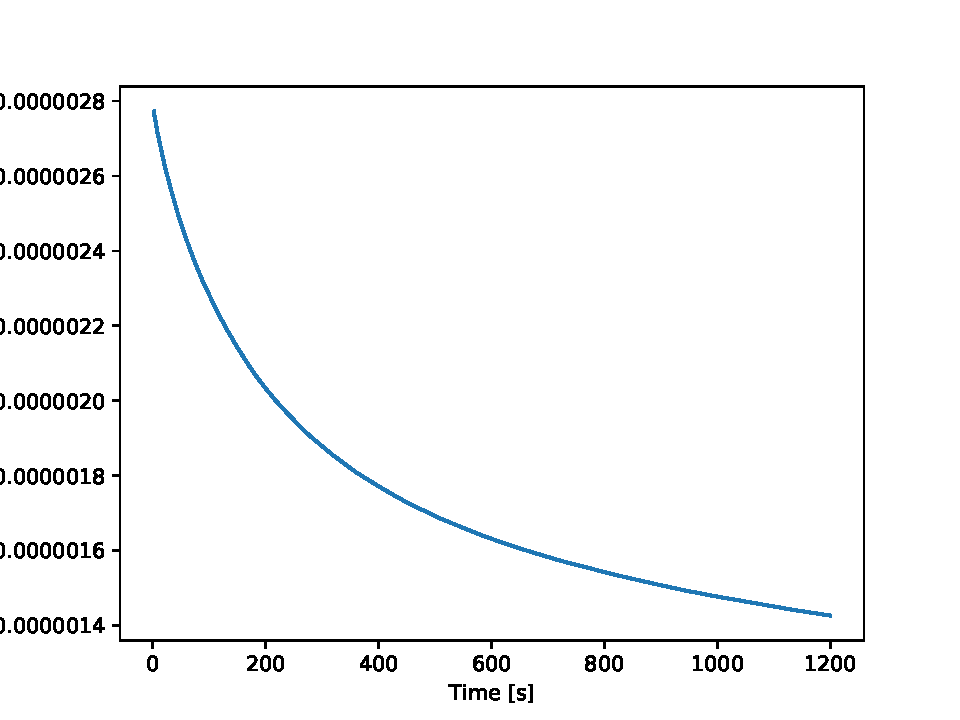
\includegraphics[scale=0.5]{figures/aml-grad-err}
    \caption{TODO Error}\label{aml:grad-err}
\end{figure}
\begin{figure}
    \centering
    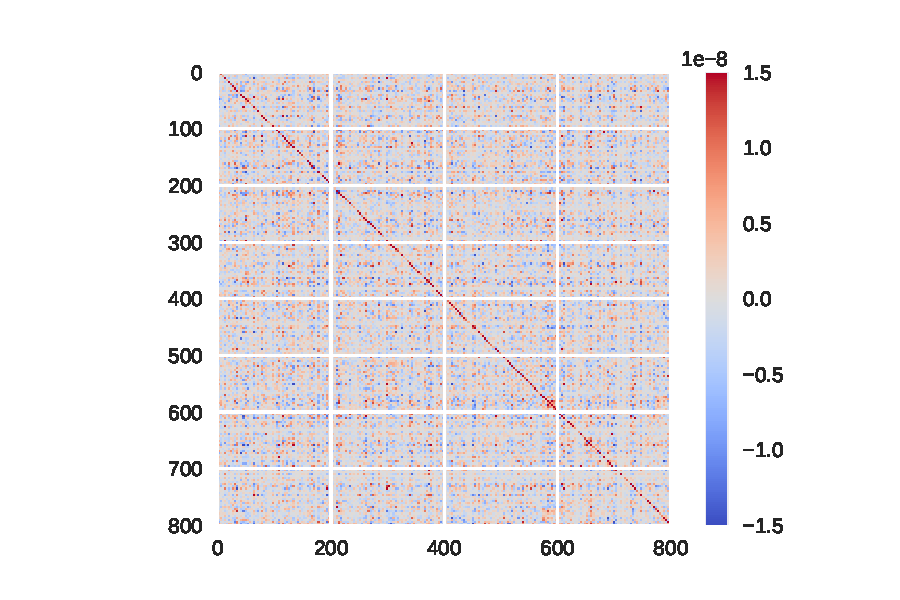
\includegraphics[scale=0.4]{figures/aml-target-weights}
    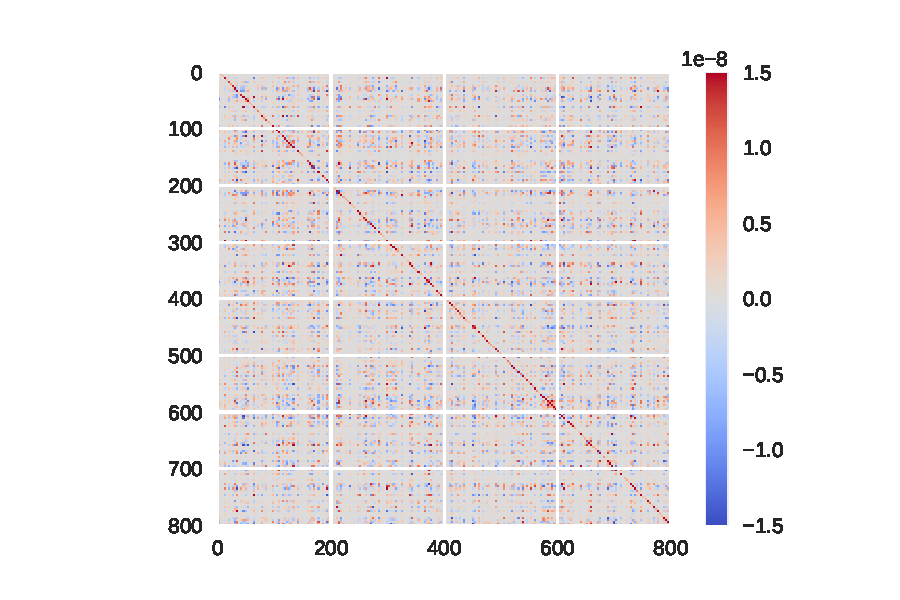
\includegraphics[scale=0.4]{figures/aml-learned-weights}
    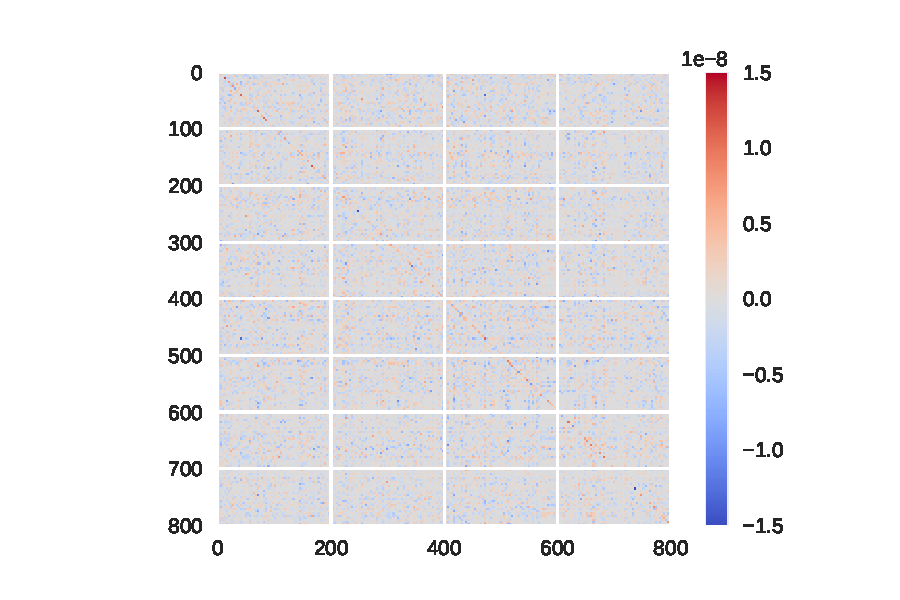
\includegraphics[scale=0.4]{figures/aml-weight-diff}
    \caption{TODO left to right: target weights, learned weights, difference}\label{aml:weights}
\end{figure}
\begin{figure}
    \centering
    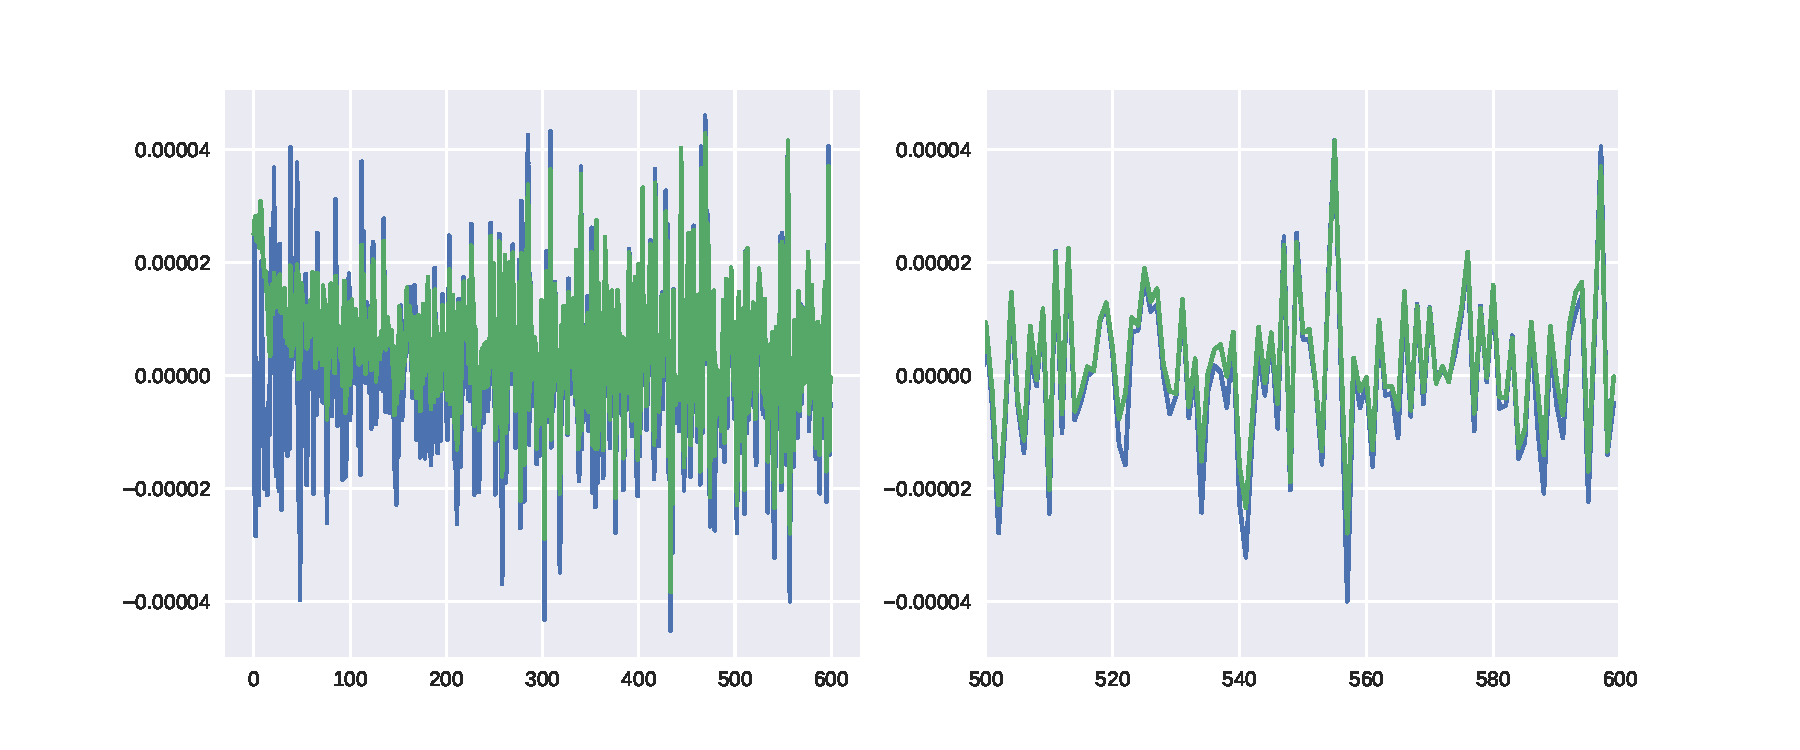
\includegraphics[scale=0.6]{figures/aml-matching-decode}
    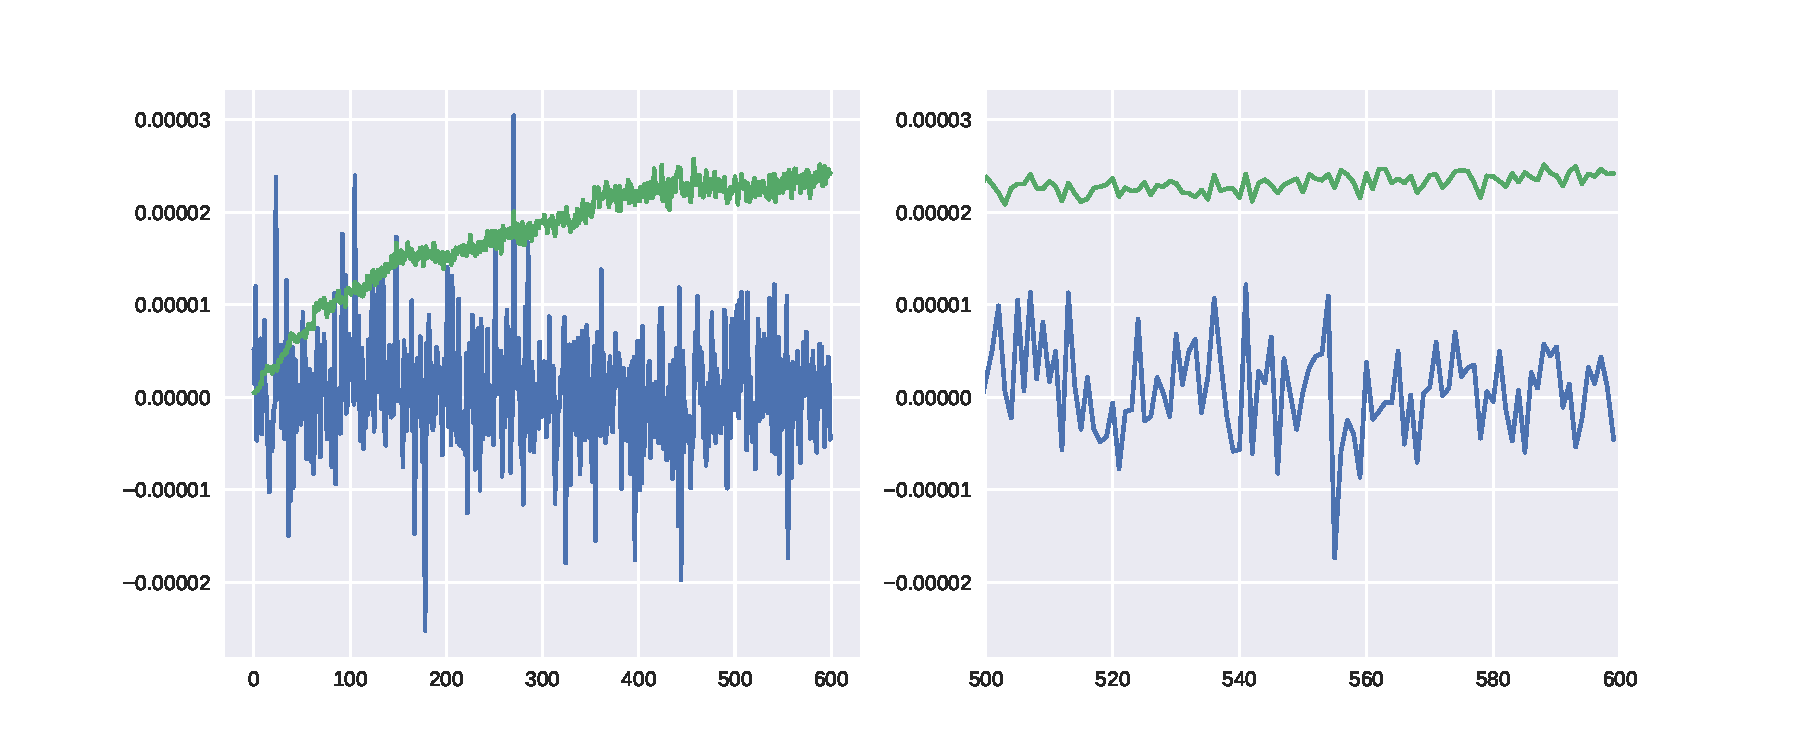
\includegraphics[scale=0.6]{figures/aml-nonmatching-decode}
    \caption{TODO two output dimensions over time (matching and non-matching)}\label{aml:grad-decode}
\end{figure}

Again, the pure derivation of a learning rule does not ensure its biological plausibility.
Thus, let us consider the individual terms in the gradient.
The term $\vc\act\Tr \mdec_* \vc\act$ is using the current decoders to decode the ensemble's activity in no way different than usually done in the NEF\@.
The decoded value is then correlated with the ensemble's activity.
The plausibility of this is somewhat unclear, but to my knowledge there is no data excluding this possibility.
In particular, the decoded value and activities could be projected to another neural ensembles (see \cref{fig:aml-grad-desc}) that calculates the inner product.
The same, a projection to neural ensemble calculating the inner product, could happen with the decoded value $\vc x$.
The existence of these standard decoders can be assumed as generally done in the NEF\@.
Alternatively, $\vc x\Tr \vc x$ could directly be decoded (as a square of the individual components all projecting into the same dimension).
\begin{figure}
    \centering
    \begin{tikzpicture}[nef]
        \graph[no placement] {
            pre [ens, at={(0, 0)}, minimum size=30] -- mod/"" [inner sep=0, minimum size=0, at={(1.5, 0)}] -> post [ens, at={(3, 0)}, minimum size=30],
            pre -> [bend left] act/"$\vc\act\Tr \mdec_* \vc\act$" [net, at={(0, 3)}],
            pre -> [bend right, "$\mdec_*$"] act,
            pre -> targetact/"$\vc x\Tr \vc x$" [net, at={(2, 3)}],
            act -> combine/"" [pnode, at={(1.5, 1)}],
            targetact -> ["-1"] combine,
            combine -> [modulatory] mod,
        };
    \end{tikzpicture}
    \caption{TODO}\label{fig:aml-grad-desc}
\end{figure}

The whole term $(\vc\act\Tr \mdec_* \vc\act - \vc x\Tr \vc x)$ is a scalar that influence all synapses.
This could be realized by a broadly acting neuro-modulator or by extensive connectivity of the neural ensembles calculating this error term.
Neither option is implausible.
The role of this gradient term seems to play a role weight normalization as it acts equally on all weights and the magnitude depends on the magnitude of the values of $\mdec_*$.
Also, without it all weight changes would always be negative.
Note that in many learning rules (TODO example) normalization factors are often criticized as implausible for requiring knowledge of the whole weight matrix at the level of a single synapse.
This critique does not apply to this learning rule.
The decoding matrix is only used to decode from the activities which require only local knowledge of the weights.
Furthermore, even considering this gradient term as implausible, there might be other ways in which the brain achieves a weight balance (TODO refs).

Finally, the term $\vc\act \vc\act\Tr$ correlates neuron activities and appears somewhat Hebbian-like.
Hebbian learning is one of the best studied ways biological systems learn.
In this form of learning pre- and post-synaptic neurons become connected when they fire in short succession.
In difference to this usual account, here two pre-synaptic neurons will connect to the same post-synaptic neuron if they fire together.
Again, the biological plausibility of this is somewhat uncertain, but cannot be outright rejected.


\section{Implicit error calculation}
The previous two implementations of the AML use minimal assumptions about the computational power of synapses.
All that is needed are additive weight changes proportional to some error signal.
However, it is not uncommon to assume that non-linearities in the synapses allow for multiplication (TODO ref).
That allows to roll the explicit outer product required in the previous two approaches into the synapses itself.
This requires the considerably less neurons as no neural populations are required for each product.

In this thesis, I am using an implementation that corresponds to this implicit error calculation.
This is mainly to reduce simulation times and is not meant as a statement that this is likely to correspond to the brain's implementation as there is not enough evidence to make such a strong claim.


\section{Normative interpretation}
While the AML cannot be outright rejected as biologically implausible, there are definitely some open questions concerning it.
Nevertheless, it should not be evaluated purely on this fact.
Many models in cognitive science, psychology, and computational neuroscience (TODO refs) assume the encoding of associations in an outer product matrix.
Ultimately, the validity of all those models depends on the possibility that the brain can learn such a matrix.
As such, the AML makes it explicit which operations have to be implemented to enable such learning.
If these turn out as either not being implemented in the brain or as not being implementable at all, it would follow that the brain has to use some other mechanism to represent associations.
Thus, the AML has merit as a normative theory, describing what the brain is ought to do, and directing research to open questions.

That being said, the AML does not make any assumption about the pre-synaptic neurons.
With such assumptions, some of the restrictions of the AML might be lessened.
For example, assuming orthogonal encoders, the decoder matrix $\mdec$ will be orthogonal too.
That in turn means that $\mdec_* = \mdec\Tr \mdec = \imat$ becomes the identity matrix which is independent of the exact decoders.
This simplifies connectivity and removes the need to learn the symmetric matrix $\mdec_*$ which alleviates some of the concerns of biological plausibility.

The dentate gyrus in the hippocampus is often assumed to pattern separation which is a form of orthogonalization.
Hence, it might be possible that the hippocampus learns associations with a form of the AML where $\mdec_*$ ends up being the identity matrix and thus simplifies the learning rule itself.


\section{Properties of the AML}
So far the considerations about the AML were purely theoretical.
Figure TODO demonstrates that an implementation of the AML can indeed learn associations in a spiking neural network.
TODO more description results

It is worth highlighting, that this learning rule allows one-shot learning, i.e.\ a single presentation of an association allows to recall it perfectly even after several other associations have been learned.
Most other learning rules exhibit destructive interference between the items in this scenario.
As an example, Figure TODO shows the same experiment using the Prescribed Error Sensitivity (PES) learning rule (TODO ref) which is commonly used in NEF models (TODO refs).
Here all associations except for the last get destroyed.
It is still possible to learn associations with PES, but it requires to present each item multiple times, i.e.\ one-shot learning cannot be done to learn associations in a reliable way.
To learn a new association, old associations need to be presented again.

This ability for one-shot learning with the AML is due to the $\mdec_*$ matrix which accounts for the interference between neurons.
In fact, the AML and PES are the same except for that matrix.
The PES learning rule can be expressed as
\begin{equation}
    \od{\tilde{\mdec}}{t} = \eta \vc v(t) \vc\act_{\vc u}\Tr(t) \text{,}
\end{equation}
while the AML learning rule can be written as
\begin{equation}
    \od{\tilde{\mdec}}{t} = \eta \vc v(t) \vc u(t)\Tr \mdec = \eta \vc v(t) \vc\act_{\vc u}\Tr(t) \mdec\Tr \mdec
\end{equation}
which is the same, except for $\mdec_* = \mdec\Tr \mdec$.

The one-short learning ability comes with some limitations, though.
The learning rule is restricted to learn transformations that can be expressed as outer product matrices, while learning rules like PES can learn arbitrary transform matrices.
Moreover, the learning rule is essentially trying to learn a look-up table mapping items to other items.
Thus, one should not expect the AML to generalize.


\section{Weight normalization}
Note that the AML allows weights to grow without bound.
By introducing a factor of $1 - \vc v(t)\Tr \hat{\vc v}(t)$ this can be prevented, but similar to other weight normalizations it introduces the need for each weight to have access to the global population activity and weights as $\hat{\vc v}(t) = \tilde{\mdec} \vc\act_{\vc u}(t)$.
Such global dependencies are ofter criticized for not being biological plausible.
As such, I decided to take a slightly different approach with an equivalent effect.
Instead of including the dot product $\vc v(t)\Tr \hat{\vc v}(t)$ in the learning rule, it can be computed by another neural population and the result can be used to inhibit the population providing $\vc v$.
Once fully inhibited $\vc\act_{\vc v}(t)$ will be all-zero and thus prevent further weight changes.


Things to mention:
\begin{itemize}
    \item Different learning rules for different things seem plausible. For example, motor learning requires many repetitions (no one-shot learning), but seems to somewhat generalize (and is continuous). So this might be done with something PES like. Fact learning (a form of associations) can be one-shot, but generalizing from multiple facts is a conscious process/does not happen automatically. This might be done with something AML like.
    \item Maybe that explains the need for consolidation? First, one shot learning that doesn't allow generalization, then in consolidation commonalities get extracted? Replay in sleep/resting might produce the interleaving/multiple presentations required to learn associations with PES\@.
    \item Gallistel argues there is no general purpose learning rule, which is in line with the more pupose specific learning rules in this chapter
\end{itemize}
